\documentclass[a4paper,11pt]{article}

\usepackage[english]{babel}
\usepackage{float}
\usepackage{graphicx}
\usepackage{amsmath,amsthm}
\usepackage{gensymb}
\usepackage{amssymb}
\usepackage[margin=2.cm]{geometry}
\usepackage{pstricks-add}	%for geometric diagrams
\usepackage{chemfig}	%for structural formulae
\usepackage{tabularx}	%for better tables
\usepackage{booktabs}	%for better tables
\usepackage[makeroom]{cancel}	%for cancelling lines
\usepackage{hyperref}	%hyperlinks
\usepackage{mathrsfs}
\usepackage{mathtools}
\usepackage{epigraph}	%quotes
\usepackage{lastpage}
\usepackage{multicol}	%column environments
\usepackage{fancyhdr}	%headers
\usepackage[at]{easylist}	%easy lists
\usepackage{wasysym}
\usepackage{wrapfig}	%wrap figures in text
\usepackage{subfig}		%subfigures
\usepackage{tikz}

\allowdisplaybreaks
\newcommand\numberthis{\addtocounter{equation}{1}\tag{\theequation}}
\setlength{\epigraphwidth}{7.7cm}
\setlength{\tabcolsep}{10pt}

% bracket group shorthands
\newcommand{\abs}[1]{\left|#1\right|}
\newcommand{\set}[1]{\left\{#1\right\}}

% common sets
\newcommand{\R}{\mathbb{R}}
\newcommand{\Cmplx}{\mathbb{C}}
\newcommand{\Q}{\mathbb{Q}}
\newcommand{\Z}{\mathbb{Z}}
\newcommand{\N}{\mathbb{N}}

% derivative shorthands
\newcommand{\diff}[2]{\frac{\mathrm{d}#1}{\mathrm{d}#2}}
\newcommand{\pdiff}[2]{\frac{\partial #1}{\partial #2}}
\newcommand{\ndiff}[3]{\frac{\mathrm{d}^{#3}#1}{\mathrm{d}#2^{#3}}}
\newcommand{\npdiff}[3]{\frac{\partial^{#3} #1}{\partial #2^{#3}}}

% theorem environments
\newtheorem*{definition*}{Definition}
\newtheorem*{lemma*}{Lemma}
\newtheorem{theorem}{Theorem}
\newtheorem*{theorem*}{Theorem}
\newtheorem*{corollary*}{Corollary}
\newtheorem{example}{Example}
\newtheorem*{remark}{Remark}

\DeclareMathOperator{\bdy}{Bdy}
\DeclareMathOperator{\interior}{Int}

% header
\pagestyle{fancy}
\lhead{Question Breakdown - Set 1, Question 5}
\rhead{Year 11 2018}

%\title{Question Breakdown - Set 1, Question 5}
%\date{\today}
%\author{Daniel Czapski}

\begin{document}
\section*{Question Breakdown - Set 1, Question 5}
Uluru is a large rock on flat ground in Central Australia. Three tourists, $A$, $B$ and $C$ are observing Uluru from the ground. $A$ is due North of Uluru, $C$ is due East of Uluru and $B$ is on the line-of-sight from $A$ to $C$ and between them\footnote{i.e. on the line from $A$ to $C$.}. The angles of elevation to the summit of Uluru from $A$, $B$ and $C$ are 26\degrees, 28\degree and 30\degree respectively.\\

\noindent Determine the bearing of $B$ from Uluru.
\subsection*{Solution}
This question combines a few major topics of study in trigonometry; in particular, bearings, non-right-angled trigonometry and 3D trigonometry. When addressing especially 3D trigonometry and bearings problems, the best place to start is with a \textbf{diagram}. In particular, ensure that your diagram 
\vspace{0.15cm}
\begin{easylist}[itemize]
@ is \textbf{large} (about half a page is sufficient);
@ \textbf{contains all the information given} in the question (in this case, the angles at $A$, $B$ and $C$);
@ \textbf{contains what you are required to find} (the bearing of $B$ from Uluru, which will involve the angle between $B$ and North);
@ if necessary, \textbf{contains other quantities that you define}; and
@ has \textbf{North labelled clearly} (if the question involves bearings).\\
\end{easylist}
\vspace{0.15cm}

\noindent Let the point $O$ be the base of Uluru and the point $S$ be the summit. We are given that $\angle SAO$, $\angle SBO$ and $\angle SCO$ are $26\degree$, $28\degree$ and $30\degree$ respectively. In addition, let $SO=h$, the height of Uluru, and $\angle AOB=\theta$, the angle between the lines from the base of Uluru to $A$ and $B$ respectively. 

\begin{center}
	\begin{tikzpicture}
	\draw (0,0) -- (9,0) -- (-3.8971,-2.25) -- cycle;
    \draw (0,0) -- (0,4.5) -- (-3.8971,-2.25);
    \draw (0,4.5) -- (9,0);
    \draw (0,0) -- (3,-1.04675) -- (0,4.5);
    \draw[->] (-0.25,1.6) -- (-0.25,0);
    \draw[->] (-0.25,2.3) -- (-0.25,3.75);
    \draw[->,very thick] (6,4) -- (7,4) node[right] {\textbf{N}};
    
    \draw (8.1056,0.445) arc (153.4:180:1);
    \draw (2.5243,-0.1672) arc (140:180:1);
    \draw (-3.3972,-1.38395) arc (30:0:1);
    \draw (1,0) arc (-30:-49:1);
    
    \node[above right] at (0,0) {$O$};
    \node[above] at (0,4.5) {$S$};
    \node[left] at (-3.8971,-2.25) {$C$};
    \node[right] at (9,0) {$A$};
    \node[below right] at (3,-1.04675) {$B$};
    
    \node at (-0.25,1.95) {$h$};
    \node at (7.4,0.4) {$26\degree$};
    \node at (-2.8,-1.2) {$30\degree$};
    \node at (3.3,-0.6) {$28\degree$};
    \node at (1.2,-0.175) {$\theta$};
	\end{tikzpicture}
\end{center}

This diagram is an isometric view of the problem. However, the angle we really want to find here is $\theta$. As this is in $\triangle AOB$, a second diagram, drawn from above, might be more illuminating. 

\begin{center}
	\begin{tikzpicture}
	\draw (0,0) -- (9,0) -- (0,-4.5) -- cycle;
    \draw (0,0) -- (3.5,-2.75);
    \draw (1,0) arc (0:-38.2:1);
    \draw[->,very thick] (7,-3) -- (8,-3) node[right] {\textbf{N}};
    \draw (0.4,0) -- (0.4,-0.4) -- (0,-0.4);
    
    \node[above left] at (0,0) {$O$};
    \node[right] at (9,0) {$A$};
    \node[below right] at (3.5,-2.75) {$B$};
    \node[below left] at (0,-4.5) {$C$};
    \node at (1.2,-0.4) {$\theta$};
	\end{tikzpicture}
\end{center}

\begin{remark}\normalfont
Draw as many diagrams from as many angles as required. Generally, an isometric diagram and a top-down diagram are the most helpful. It can sometimes also be helpful to draw separate diagrams of each individual triangle in a problem.
\end{remark}

\noindent Looking at our second diagram, it is likely that we will need to focus on determining angles in the (non-right-angled) $\triangle AOB$; the sine or cosine rules are likely to be involved in this process. However, in order to do this, we will need useful expressions for at least some of the side lengths -- at the very least, $AO$ and $BO$, and possibly $CO$ as well. Since we have not been given any lengths explicitly we can't really give exact values for these lengths. However, looking back at the first diagram, we can express them in terms of the angle of elevation to the summit and the height $h$.\\

\noindent Another way to think about this is to note that we really should use all the information in the question, and the easiest way to relate the angles of elevation to the distances of $A$, $B$ and $C$ from the base $O$ is through the height $h$.\\

\noindent Examining triangles $SOC$, $SOB$ and $SOA$, we have
\begin{align*}
\tan(30\degree) = \frac{h}{CO} && \tan(28\degree) = \frac{h}{BO} && \tan(26\degree) = \frac{h}{AO}\\
CO = h\cot(30\degree) && BO = h\cot(28\degree) && AO = h\cot(26\degree).
\end{align*}

\noindent Let's put this information on the diagram and see what we have.

\begin{center}
	\begin{tikzpicture}
	\draw (0,0) -- (9,0) -- (0,-4.5) -- cycle;
    \draw (0,0) -- (3.5,-2.75);
    \draw (1,0) arc (0:-38.2:1);
    \draw[->,very thick] (7,-3) -- (8,-3) node[right] {\textbf{N}};
    \draw (0.4,0) -- (0.4,-0.4) -- (0,-0.4);
    
    \node[above left] at (0,0) {$O$};
    \node[right] at (9,0) {$A$};
    \node[below right] at (3.5,-2.75) {$B$};
    \node[below left] at (0,-4.5) {$C$};
    \node at (1.2,-0.4) {$\theta$};
    
    \node at (-1,-2.25) {$h\cot(30\degree)$};
    \node at (2.75,-1.25) {$h\cot(28\degree)$};
    \node at (4.5,0.25) {$h\cot(26\degree)$};
	\end{tikzpicture}
\end{center}

\begin{remark}\normalfont
It is often helpful to put important information gained during your working out on diagrams. You can append it to diagrams you have already drawn, though if them start to become too cluttered feel free to draw additional diagrams. 
\end{remark}

The $\cot$ ratios have known values (since the angles are known), so it is just $h$ that is unknown in these expressions. In order to evaluate anything, therefore, we need to be able to eliminate any $h$ appearing in the expression. Combinations of the sine and cosine rule in $\triangle AOB$ will always involve at least two unknowns (not including $h$), so this isn't a productive line of inquiry just yet. However, we also have the triangle $AOC$, which is right-angled. In particular, we have expressions for the sides that are adjacent and opposite to the angle $OAC$. So, we can write

\begin{align*}
\tan(\angle AOC) &= \frac{CO}{AO}\\
&= \frac{h\cot(30\degree)}{h\cot(26\degree)}\\
%&= \frac{\tan(26\degree)}{\tan(30\degree)}\\
&= 0.844778\ldots
\end{align*}
We know that $\tan$ is positive in the first and third quadrants, however $\angle OAC$ is an interior angle of a right-angled triangle, thus it must be acute, so we take the acute solution (which coincides with $\tan^{-1}(0.844778)$ on your calculator\footnote{This is because the range of the inverse tan function is $-90\degree < y < 90\degree.$}):

$$
\implies \angle OAC =\ \sim 40.19\degree
$$

\begin{remark}\normalfont 
It is likely that we will use this quantity again in a calculation. To prevent rounding errors it is good practice to save intermediate quantities such as these as exactly as possible. The best way to do this is to use the memory buttons on your calculator (see your calculator's user manual for details). 
\end{remark}

\noindent Let's put this on the diagram as well.

\begin{center}
	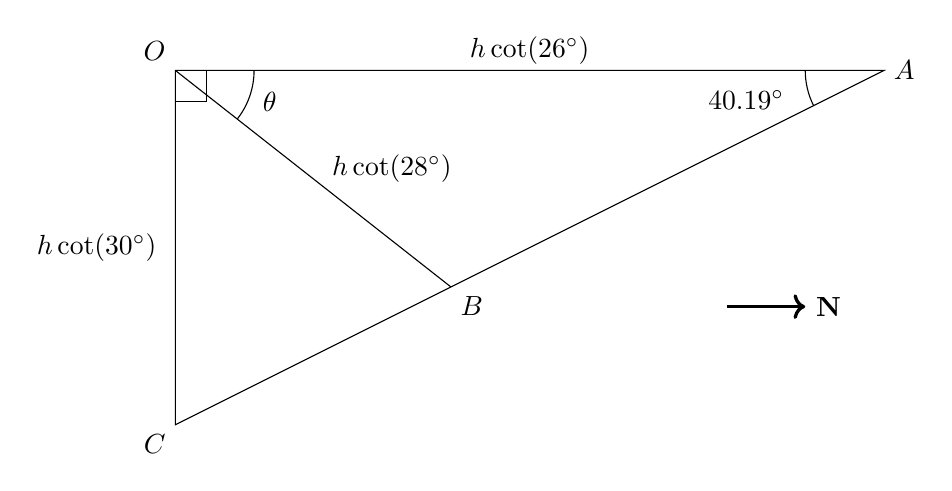
\begin{tikzpicture}
	\draw (0,0) -- (9,0) -- (0,-4.5) -- cycle;
    \draw (0,0) -- (3.5,-2.75);
    \draw (1,0) arc (0:-38.2:1);
    \draw[->,very thick] (7,-3) -- (8,-3) node[right] {\textbf{N}};
    \draw (0.4,0) -- (0.4,-0.4) -- (0,-0.4);
    
    \draw (8,0) arc (180:206.56:1);
    
    \node[above left] at (0,0) {$O$};
    \node[right] at (9,0) {$A$};
    \node[below right] at (3.5,-2.75) {$B$};
    \node[below left] at (0,-4.5) {$C$};
    \node at (1.2,-0.4) {$\theta$};
    
    \node at (-1,-2.25) {$h\cot(30\degree)$};
    \node at (2.75,-1.25) {$h\cot(28\degree)$};
    \node at (4.5,0.25) {$h\cot(26\degree)$};
    \node at (7.25,-0.375) {$40.19\degree$};
	\end{tikzpicture}
\end{center}

\noindent Remember, we still want to find $\theta$: the sine and cosine rules in $\triangle AOB$ are the main methods for doing so. However, the sine and cosine rules involving $\theta$ still contain two unknowns -- the fact that we don't know the length on $AB$ is problematic to this approach. But if we can find $\angle OBA$, then we can take advantage of the angle sum of a triangle to determine $\theta$. The cosine rule is not an option since we don't know $AB$ \footnote{Strictly speaking, we can use the cosine rule to find an expression for $AB$ in terms of $h$, and then use this to determine $\theta$ using the sine or cosine rule directly, but this is somewhat more difficult.}, so the sine rule is probably the most useful tool we have remaining. In particular, we can write

\begin{align*}
\frac{\sin(\angle OBA)}{AO} &= \frac{\sin(\angle BAO)}{OB}\\
\frac{\sin(\angle OBA)}{h\cot(26\degree)} &= \frac{\sin(40.19\ldots \degree)}{h\cot(28\degree)}\\
\sin(\angle OBA) &= \frac{\sin(40.19\ldots\degree)\tan(28\degree)}{\tan(26\degree)}\\
&= 0.703516\ldots 
\end{align*}

\noindent Now, sine is positive in both the first and second quadrants, so either solution is potentially an angle in a triangle (as they are both less than 180\degree). However, if we were to take the acute (first quadrant solution), then $\theta$ would be larger than $90\degree$, which contradicts the fact that $B$ is on the line-of-sight from $A$ to $C$ and between them (as stated in the question) -- this would mean $B$ was on the other side of $C$ (see the diagram). So we must take the obtuse (second quadrant) solution (which does NOT coincide with $\sin^{-1}(0.703516\ldots)$!):

$$
\angle OBA =\ \sim 134.71\degree.
$$

%\noindent For the sake of completeness and consistency, we will put this on the diagram as well. 

\noindent We know that the angle sum of a triangle is $180\degree$, so $\theta = 180-\angle OAB - \angle OBA =\ \sim 5.1\degree$. The question asked for a bearing, so we may conclude that the point $B$ is on a bearing of $5\degree T$ (5\degree\ true) or $N5\degree E$ from Uluru.

\vspace{2cm}

If you desire formal tutoring in Preliminary or HSC English, two, three or four units of Mathematics, Science or Economics, Talent 100 offers a comprehensive, structured course taught by a combination of the top HSC achievers of past years, qualified and experienced teachers and leading textbook authors. For HSC success, simplified, contact us on 1300 999 100, check out our website at \url{https://talent-100.com.au/} and find us on Facebook. 

\vfill

\begin{figure}[H]
\centering

\includegraphics[width=0.17\textwidth]{t100.png}
\end{figure}

\end{document}